\chapter{Zielsetzung und Vorgehensweise} 

\section{Zielsetzung}

Das Projektziel ist die Entwicklung eines Systems, welches automatisiert EPLAN-Artikel \parencite{EPLANArtikelverwaltung} zu EPLAN-Fenstermakros \parencite{EPLAN-Makros} zuordnet.
Für einen vorhanden technischen EPLAN-Artikel \parencite{EPLANArtikelverwaltung} soll anhand einer technischen Anfrage (zum Beispiel in Form eines Datenblatts) das fachlich passendste EPLAN-Fenstermakro \parencite{EPLAN-Makros} identifiziert werden.


Diese Problemstellung kann als Rankingaufgabe formuliert werden, bei der für jede Anfrage eine Menge bekannter EPLAN-Fenstermakros \parencite{EPLAN-Makros} vorliegt. Dabei sind alle Kandidaten dieser Menge potenzielle Ergebnisse für den 1. Rang.
Das System soll die Eigenschaften eines gegebenen EPLAN-Artikels \parencite{EPLANArtikelverwaltung} analysieren und diese mit allen verfügbaren Makro-Kandidatenprofilen vergleichen. Anschließend sollen die Kandidaten entsprechend ihrer Relevanz geordnet werden.
Ziel dabei ist es, dass das passendste EPLAN-Fenstermakro \parencite{EPLAN-Makros} möglichst auf Rang 1 erscheint. Die weniger ähnlichen Kandidaten sollen entsprechend der Bewertung hierarchisch auf den nachfolgenden Rängen einsortiert werden.


Im Gegensatz zu Klassifikationsaufgaben liegt der Fokus dieses Systems nicht direkt auf der Bestimmung einer einzelnen Klasse oder Produktfamilie. Vielmehr geht es darum eine möglichst präzise Variantenauflösung zu erreichen.
Dafür sollen die technischen Eigenschaften und Merkmale aus einer Anfrage systematisch erfasst und mit den Eigenschaften der EPLAN-Artikel \parencite{EPLANArtikelverwaltung} abgeglichen werden.


Die Herausforderung besteht darin, dass sich viele Produkte lediglich in einzelnen technischen Eigenschaften und Konfigurationsmerkmalen unterscheiden. Geringe Abweichungen können deshalb zu unterschiedlichen Makrozuordnungen führen.
Das System muss daher in der Lage sein allgemeine technischen Zusammenhänge als auch merkmalspezifische Unterschiede zwischen ähnlichen Varianten zu erkennen.


Zur Lösung dieses Problems wird ein Learning-to-Rank-System entwickelt, welches strukturierte technische sowie lexikalische Merkmale aus Artikeldaten kombiniert, um die Relevanz von potenziellen EPLAN-Fenstermakros \parencite{EPLAN-Makros} zu bewerten. 
Das Modell erzeugt für jeden verfügbaren Makrokandidaten eine Relevanzbewertung und erstellt daraus eine Rangliste möglicher Empfehlungen. Ziel ist es, das korrekte Zielmakro möglichst auf den vorderen Rangpositionen, idealerweise auf Rang 1, zu platzieren.

\section{Methodisches Vorgehen}

Das methodische Vorgehen orientiert sich an der \textit{Design Science Research Methodology} (DSRM) nach Peffers et al. \citeyearpar{peffers2007dsrm}. 
Die DSRM beschreibt einen strukturierten Forschungsprozess zur Entwicklung und Evaluation technischer Artefakte und eignet sich insbesondere für die Entwicklung von IT-Systemen.
Das Ziel der Methodik besteht darin, eine konkrete Problemstellung systematisch zu analysieren, ein geeignetes Artefakt zu entwickeln und den Nutzen durch eine Evaluation nachzuweisen. 

Der von Peffers et al. beschriebene Forschungsprozess umfasst die folgenden Schritte: 

\begin{enumerate} 
    \item Problemidentifikation und Motivation 
    \item Definition der Lösungsziele 
    \item Design und Entwicklung des Artefakts 
    \item Demonstration der entwickelten Lösung 
    \item Evaluation des Artefakts 
    \item Kommunikation der Ergebnisse 
\end{enumerate} 

In dieser Arbeit bildet die DSRM den übergeordneten Rahmen. Die iterative Entwicklung des Ranking-Systems erfolgt innerhalb der Design-, Entwicklungs- und Evaluationsphase durch wiederkehrende Entwicklungszyklen. 

\section{Iterativer Entwicklungsprozess} 

Zur Entwicklung des Artefakts wird die Design-Science-Methodik durch die Prinzipien des \textit{Action Design Research} (ADR) nach Sein et al. verwendet \citeyearpar{sein2011adr}. 
ADR verbindet dabei die Entwicklung eines Artefakts mit der fortlaufenden Anwendung, Evaluation und Verbesserung. 
Während die DSRM den strukturellen Prozess beschreibt, liefert ADR den Entwicklungszyklus zur kontinuierlichen Verbesserung des Systems. 

Der iterative Entwicklungsprozess besteht dabei aus den folgenden Schritten: 

\begin{enumerate} 
    \item Analyse des aktuellen Zustands und Identifikation von Verbesserungspotentialen 
    \item Recherche wissenschaftlicher und technischer Lösungen
    \item Konzeption neuer Komponenten, Merkmale oder Optimierungen
    \item Implementierung und Anpassung der entwickelten Ansätze 
    \item Durchführung von Tests und Validierungen 
    \item Evaluation anhand definierter Qualitätsmetriken 
    \item Interpretation der Ergebnisse 
    \item Ableitung weiterer Verbesserungen
\end{enumerate} 

Die Ergebnisse einer Iteration bilden jeweils die Grundlage für die nachfolgenden Iterationen. Auf diese Weise entsteht ein kontinuierlicher Verbesserungsprozess, in dem Forschung, Entwicklung, Evaluation und Optimierung miteinander verzahnt sind. 
Die Kombination aus DSRM und ADR ermöglicht somit auf der einen Seite einen strukturierten Forschungsprozess und auf der anderen Seite eine iterative Verbesserung des entwickelten Ranking-Systems. 
Abbildung \ref{fig:dsrm_adr_verzahnung} veranschaulicht diese Verzahnung der beiden Methodiken.

Die theoretischen Grundlagen der verwendeten Bewertungsmetriken wurden bereits in Kapitel \ref{chap:stand_der_technik} vorgestellt. 
Die Anwendung dieser Metriken zur Bewertung des entwickelten Systems erfolgt in Kapitel \ref{chap:evaluierungskonzept}.
Eine Darstellung der finalen Systemarchitektur und der vollständigen Pipeline befindet sich ebenfalls in diesem Kapitel.


\begin{figure}[tbp]
    \centering
    \resizebox{\textwidth}{!}{%
    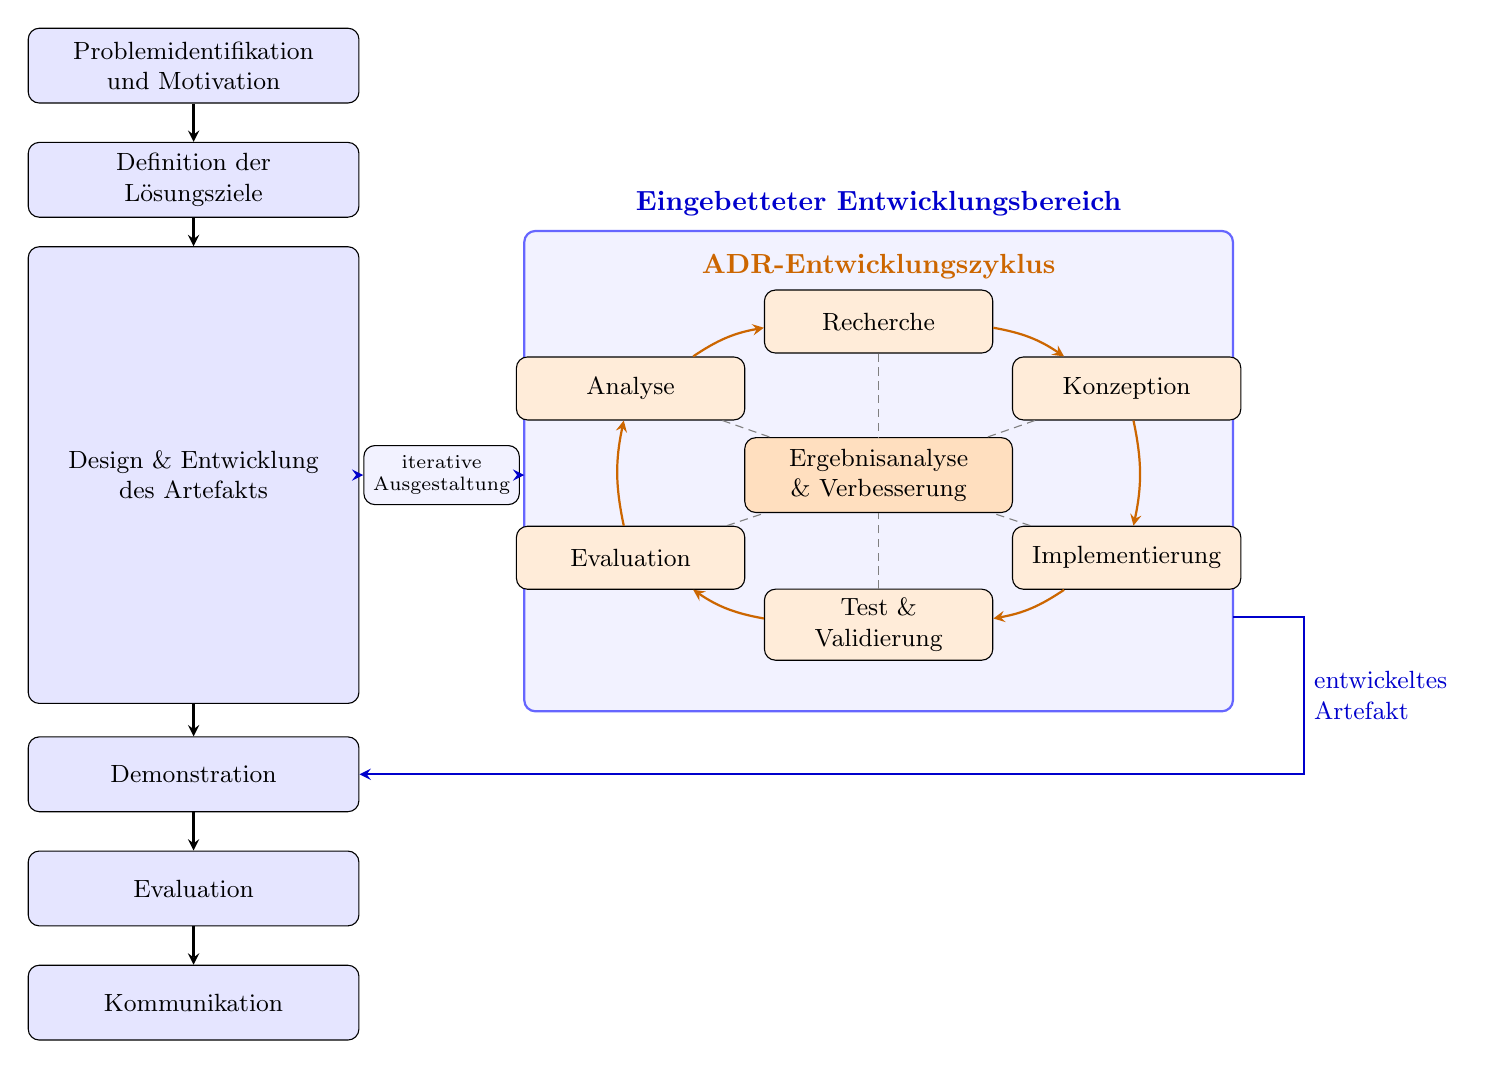
\begin{tikzpicture}[
        >=stealth,
        font=\small,
        dsrm/.style={draw, rounded corners, fill=blue!10, minimum width=4.2cm, minimum height=0.95cm, align=center},
        adr/.style={draw, rounded corners, fill=orange!15, minimum width=2.9cm, minimum height=0.8cm, align=center},
        analysis/.style={draw, rounded corners, fill=orange!25, minimum width=3.4cm, minimum height=0.95cm, align=center},
        bridge/.style={draw, rounded corners, fill=blue!5, minimum width=1.8cm, minimum height=0.75cm, align=center, font=\scriptsize},
        flow/.style={->, thick},
        cycle/.style={->, thick, orange!80!black},
        relation/.style={densely dashed, gray},
        artifact/.style={->, thick, blue!80!black}
    ]

        \node[dsrm] (problem) at (0, 0) {Problemidentifikation\\und Motivation};
        \node[dsrm] (goals) at (0, -1.45) {Definition der\\Lösungsziele};
        \node[dsrm, minimum height=5.8cm] (designphase) at (0, -5.2) {Design \& Entwicklung\\des Artefakts};
        \node[dsrm] (demo) at (0, -9.0) {Demonstration};
        \node[dsrm] (eval) at (0, -10.45) {Evaluation};
        \node[dsrm] (comm) at (0, -11.9) {Kommunikation};

        \draw[flow] (problem) -- (goals);
        \draw[flow] (goals) -- (designphase);
        \draw[flow] (designphase) -- (demo);
        \draw[flow] (demo) -- (eval);
        \draw[flow] (eval) -- (comm);

        \draw[blue!60, thick, rounded corners, fill=blue!5]
            (4.2, -2.1) rectangle (13.2, -8.2);
        \node[font=\bfseries, text=blue!80!black, align=center] at (8.7, -1.75)
            {Eingebetteter Entwicklungsbereich};

        \node[font=\bfseries, text=orange!80!black] at (8.7, -2.55)
            {ADR-Entwicklungszyklus};
        \node[adr] (analyse) at (5.55, -4.1) {Analyse};
        \node[adr] (recherche) at (8.7, -3.25) {Recherche};
        \node[adr] (konzeption) at (11.85, -4.1) {Konzeption};
        \node[adr] (implement) at (11.85, -6.25) {Implementierung};
        \node[adr] (test) at (8.7, -7.1) {Test \&\\Validierung};
        \node[adr] (adreview) at (5.55, -6.25) {Evaluation};
        \node[analysis] (improve) at (8.7, -5.2) {Ergebnisanalyse\\\& Verbesserung};

        \draw[cycle] (analyse) to[bend left=12] (recherche);
        \draw[cycle] (recherche) to[bend left=12] (konzeption);
        \draw[cycle] (konzeption) to[bend left=12] (implement);
        \draw[cycle] (implement) to[bend left=12] (test);
        \draw[cycle] (test) to[bend left=12] (adreview);
        \draw[cycle] (adreview) to[bend left=12] (analyse);

        \foreach \n in {analyse,recherche,konzeption,implement,test,adreview} {
            \draw[relation] (\n) -- (improve);
        }

        \node[bridge] (iteration) at (3.15, -5.2) {iterative\\Ausgestaltung};
        \draw[artifact] (designphase.east) -- (iteration.west);
        \draw[artifact] (iteration.east) -- (4.2, -5.2);
        \draw[artifact] (13.2, -7.0) -- ++(0.9, 0) |- node[pos=0.25, right, align=left] {entwickeltes\\Artefakt} (demo.east);

    \end{tikzpicture}%
    }

    \caption{Verzahnung von DSRM und ADR. Die DSRM bildet den übergeordneten Forschungsrahmen, während ADR als iterativer Entwicklungszyklus innerhalb der Phase \glqq Design \& Entwicklung des Artefakts\grqq\ eingesetzt wird.}
    \label{fig:dsrm_adr_verzahnung}
\end{figure}










